\documentclass[conference]{IEEEtran}
\IEEEoverridecommandlockouts
\usepackage{cite}
\usepackage{amsmath,amssymb,amsfonts}
\usepackage{graphicx}
\usepackage{textcomp}
\usepackage{xcolor}
\usepackage[utf8]{inputenc}
\usepackage[T1]{fontenc}
\usepackage{booktabs}
\usepackage{tikz}
\usetikzlibrary{shapes.geometric,positioning}
\def\BibTeX{{\rm B\kern-.05em{\sc i\kern-.025em b}\kern-.08em
    T\kern-.1667em\lower.7ex\hbox{E}\kern-.125emX}}

\tikzset{
  bloco/.style={rectangle, rounded corners=2pt, draw=black!70, fill=blue!5,
    text width=0.82\columnwidth, align=center, minimum height=6.5mm, font=\footnotesize},
  termo/.style={ellipse, draw=black!70, fill=black!8,
    text width=0.6\columnwidth, align=center, minimum height=6mm, font=\footnotesize},
  seta/.style={->, thick, draw=black!60}
}

\begin{document}

\title{Previsão de Preço de Carros Usados com Técnicas de Aprendizado de Máquina e Mineração de Dados}

\author{%
\begin{tabular}{cc}
\begin{minipage}[b]{0.42\linewidth}\centering
{\large Luis Ricardo Santos}\\[0.4em]
\textit{Programa de Pós-Graduação} \\
\textit{Universidade Federal de Itajubá (UNIFEI)}\\
Itajubá, Brasil \\
luis.ricardo@unifei.edu.br
\end{minipage}
&
\begin{minipage}[b]{0.42\linewidth}\centering
{\large Anderson Candido Alves}\\[0.4em]
\textit{Programa de Pós-Graduação} \\
\textit{Universidade Federal de Itajubá (UNIFEI)}\\
Itajubá, Brasil \\
anderson.alves@unifei.edu.br
\end{minipage}
\\[2.5em]
\begin{minipage}[b]{0.42\linewidth}\centering
{\large Gabriel Leal dos Santos}\\[0.4em]
\textit{Programa de Pós-Graduação} \\
\textit{Universidade Federal de Itajubá (UNIFEI)}\\
Itajubá, Brasil \\
gabrielleal@unifei.edu.br
\end{minipage}
&
\begin{minipage}[b]{0.42\linewidth}\centering
{\large Rafael Fernandes Pereira}\\[0.4em]
\textit{Programa de Pós-Graduação} \\
\textit{Universidade Federal de Itajubá (UNIFEI)}\\
Itajubá, Brasil \\
rafael.fernandes@unifei.edu.br
\end{minipage}
\end{tabular}%
}

\maketitle

\begin{abstract}
A precificação de veículos usados é um problema de regressão de elevada relevância econômica, marcado por relações não lineares entre idade, quilometragem e especificações mecânicas. Neste trabalho, técnicas de aprendizado de máquina e mineração de dados foram aplicadas para prever o preço de venda de carros usados a partir de um conjunto de dados real do mercado indiano, composto por 8.128 anúncios. Após limpeza, engenharia de atributos e análise exploratória apoiada por Análise de Componentes Principais, o preço foi modelado em escala logarítmica e seis algoritmos foram comparados por validação cruzada de cinco dobras com partição agrupada pelo veículo, de modo a impedir vazamento de informação. Os métodos de comitê obtiveram o melhor desempenho; o XGBoost foi o mais acurado, com coeficiente de determinação de 0,916 no conjunto de teste e erro percentual absoluto médio de 16,2 por cento, superando de forma estatisticamente significativa o gradient boosting. A interpretação por permutação indicou que o ano do veículo, a potência e o torque são os preditores mais relevantes. Demonstra-se, assim, um fluxo metodológico completo, robusto e transferível para problemas tabulares de precificação.
\end{abstract}

\begin{IEEEkeywords}
aprendizado de máquina, regressão, XGBoost, floresta aleatória, validação cruzada, mineração de dados, precificação
\end{IEEEkeywords}

\section{Introdução}

\subsection{Contexto}
A avaliação do preço de veículos usados é uma atividade economicamente significativa, presente em concessionárias, plataformas de anúncios e instituições financeiras. O preço de um automóvel usado resulta da interação de múltiplos fatores --- idade, quilometragem rodada, especificações técnicas, marca e condições de mercado --- que se relacionam de forma predominantemente não linear. Erros sistemáticos de precificação acarretam prejuízo financeiro direto, seja pela subavaliação de um ativo, seja pela perda de competitividade quando o preço é superestimado. Nesse cenário, modelos preditivos automáticos oferecem apoio à decisão consistente e escalável.

\subsection{Objetivos}
O objetivo principal deste trabalho, desenvolvido no âmbito da disciplina de Aprendizado de Máquina e Mineração de Dados \cite{pco213}, é desenvolver e comparar modelos preditivos capazes de estimar o preço de venda de carros usados a partir de suas características. Como objetivos secundários, destacam-se: (i) comparar sistematicamente seis algoritmos de naturezas distintas; (ii) avaliar o efeito da transformação logarítmica da variável-alvo; (iii) otimizar os hiperparâmetros e mitigar o vazamento de informação por meio de partição agrupada; e (iv) interpretar de forma robusta quais atributos mais influenciam a previsão.

\subsection{Perguntas de Pesquisa}
A investigação é orientada por três perguntas de pesquisa: \textbf{(PP1)} em que medida atributos de idade e de especificação mecânica explicam o preço de carros usados? \textbf{(PP2)} modelos de comitê superam um \textit{baseline} linear e métodos baseados em vizinhança neste domínio tabular, e em que magnitude? \textbf{(PP3)} qual é o compromisso entre acurácia, estabilidade de generalização e custo computacional entre os modelos avaliados?

\section{Revisão Bibliográfica}

\subsection{Fundamentação Teórica}
A previsão de preço configura uma tarefa de regressão supervisionada, na qual se busca uma função que mapeie atributos de entrada em um valor contínuo. A regressão linear constitui o \textit{baseline} clássico, assumindo relação aditiva entre preditores e resposta \cite{hastie}. Métodos baseados em vizinhança, como o $k$-vizinhos mais próximos, estimam o valor de uma amostra pela média ponderada das $k$ instâncias mais similares,
\begin{equation}
\hat{y}(\mathbf{x}) = \frac{\sum_{j \in N_k(\mathbf{x})} w_j\, y_j}{\sum_{j \in N_k(\mathbf{x})} w_j}, \quad w_j = \frac{1}{d(\mathbf{x}, \mathbf{x}_j)}, \label{eq:knn}
\end{equation}
em que $N_k(\mathbf{x})$ é o conjunto dos $k$ vizinhos e $d(\cdot)$ a distância; o método não impõe forma funcional, mas degrada-se em espaços de alta dimensão.

Os métodos de comitê (\textit{ensemble}) combinam múltiplos estimadores para reduzir o erro. A floresta aleatória \cite{breiman} emprega \textit{bagging} e amostragem aleatória de atributos para construir $B$ árvores descorrelacionadas $T_b$, cuja média reduz a variância do preditor,
\begin{equation}
\hat{y}(\mathbf{x}) = \frac{1}{B}\sum_{b=1}^{B} T_b(\mathbf{x}). \label{eq:rf}
\end{equation}
O \textit{gradient boosting} \cite{friedman} ajusta árvores rasas $h_m$ de forma sequencial, cada uma corrigindo os resíduos da anterior, atacando principalmente o viés,
\begin{equation}
F_M(\mathbf{x}) = \sum_{m=1}^{M} \nu\, \gamma_m\, h_m(\mathbf{x}), \label{eq:gb}
\end{equation}
em que $\nu$ é a taxa de aprendizado e $\gamma_m$ o peso de cada árvore. O XGBoost \cite{chen2016} é uma implementação otimizada do \textit{boosting} que acrescenta regularização explícita e amostragem de atributos, frequentemente apontada como estado da arte em dados tabulares. A Análise de Componentes Principais é amplamente utilizada na etapa exploratória para revelar a estrutura de covariância e a redundância entre atributos \cite{hastie}.

\subsection{Trabalhos Relacionados}
A previsão de preço de veículos usados tem sido investigada com diversas abordagens. Em \cite{itm2025}, comparam-se regressão linear, floresta aleatória e XGBoost, com vantagem dos métodos baseados em \textit{boosting}. De forma semelhante, \cite{preowned2023} avalia regressão linear, LASSO, árvore de decisão, floresta aleatória e \textit{boosting} extremo, reportando os comitês como mais acurados. Estudos dedicados ao XGBoost \cite{revolution} e à floresta aleatória \cite{howmuch} confirmam o bom desempenho dos métodos de árvore neste domínio, enquanto \cite{mobileapp2022} integra tais modelos em uma aplicação de precificação. Trabalhos de mineração de dados corroboram a relevância de atributos como quilometragem, marca e cilindrada \cite{ritthesis}.

\subsection{Lacuna Identificada}
A literatura concentra-se majoritariamente na comparação de acurácia entre algoritmos, dedicando menor atenção à análise conjunta da estabilidade de generalização, da significância estatística das diferenças entre modelos e das ressalvas metodológicas da interpretação por importância de variáveis. Sobretudo, raramente se controla o vazamento de informação decorrente de veículos idênticos presentes simultaneamente em treino e teste. Este trabalho busca preencher tais lacunas ao integrar, em um mesmo fluxo reprodutível, a partição agrupada, o ajuste de hiperparâmetros, a comparação por validação cruzada com teste estatístico e a interpretação por permutação.

\section{Metodologia}

\subsection{Dados}
Utilizou-se o conjunto de dados \textit{Car details v3}, de domínio público, contendo 8.128 anúncios de carros usados no mercado indiano \cite{cardekho}. As variáveis originais incluem o nome do veículo, o ano, o preço de venda, a quilometragem, o tipo de combustível, o tipo de vendedor, a transmissão, o número de proprietários anteriores, o consumo, a cilindrada, a potência e o torque.

O pré-processamento, sintetizado no fluxograma da Fig.~\ref{fig:pipeline}, seguiu etapas encadeadas. Inicialmente, 1.202 registros duplicados foram removidos, restando 6.926. Em seguida, realizou-se engenharia de atributos: a marca e o modelo foram extraídos do nome do veículo, e os campos textuais de consumo, cilindrada, potência e torque foram convertidos em valores numéricos. O tratamento de \textit{outliers} eliminou registros fora dos percentis 1 e 99 de preço e de quilometragem, bem como veículos anteriores a 1990, resultando em \textbf{6.663 amostras}. Os valores ausentes foram imputados pela mediana, no caso das variáveis numéricas, e pela moda, no caso das categóricas. Por fim, as variáveis categóricas foram codificadas pela técnica \textit{One-Hot} e as numéricas foram padronizadas pelo escore-$z$. Todas as transformações foram ajustadas exclusivamente sobre o conjunto de treino, evitando vazamento de informação durante a validação cruzada.

\begin{figure}[t]
\centering
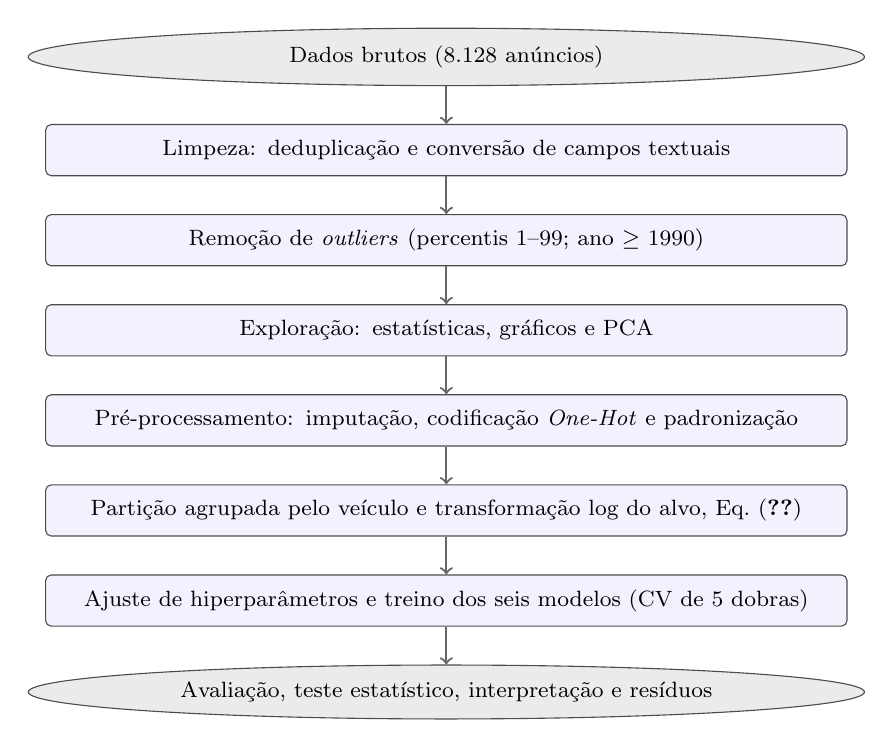
\begin{tikzpicture}[node distance=4.8mm]
\node[termo] (a) {Dados brutos (8.128 anúncios)};
\node[bloco, below=of a] (b) {Limpeza: deduplicação e conversão de campos textuais};
\node[bloco, below=of b] (c) {Remoção de \textit{outliers} (percentis 1--99; ano $\geq$ 1990)};
\node[bloco, below=of c] (d) {Exploração: estatísticas, gráficos e PCA};
\node[bloco, below=of d] (e) {Pré-processamento: imputação, codificação \textit{One-Hot} e padronização};
\node[bloco, below=of e] (f) {Partição agrupada pelo veículo e transformação log do alvo, Eq.~\eqref{eq:logtarget}};
\node[bloco, below=of f] (g) {Ajuste de hiperparâmetros e treino dos seis modelos (CV de 5 dobras)};
\node[termo, below=of g] (i) {Avaliação, teste estatístico, interpretação e resíduos};
\draw[seta] (a)--(b); \draw[seta] (b)--(c); \draw[seta] (c)--(d);
\draw[seta] (d)--(e); \draw[seta] (e)--(f); \draw[seta] (f)--(g); \draw[seta] (g)--(i);
\end{tikzpicture}
\caption{Diagrama geral da proposta: fluxo metodológico da previsão de preço, da aquisição dos dados à interpretação dos resultados.}
\label{fig:pipeline}
\end{figure}

\subsection{Análise Exploratória}
A análise exploratória, sintetizada na Fig.~\ref{fig:eda}, revelou que a distribuição do preço é fortemente assimétrica à direita, com mediana de INR\,400 mil inferior à média de INR\,484 mil --- o que motiva a transformação logarítmica adotada na modelagem, cujo histograma resultante é aproximadamente simétrico. O preço cresce com o ano do veículo e a matriz de correlação evidencia associação positiva forte entre preço, potência e torque, e associação negativa com a quilometragem. Observa-se ainda elevada correlação mútua entre os atributos de motor, o que antecipa redundância de informação.

\begin{figure}[t]
\centerline{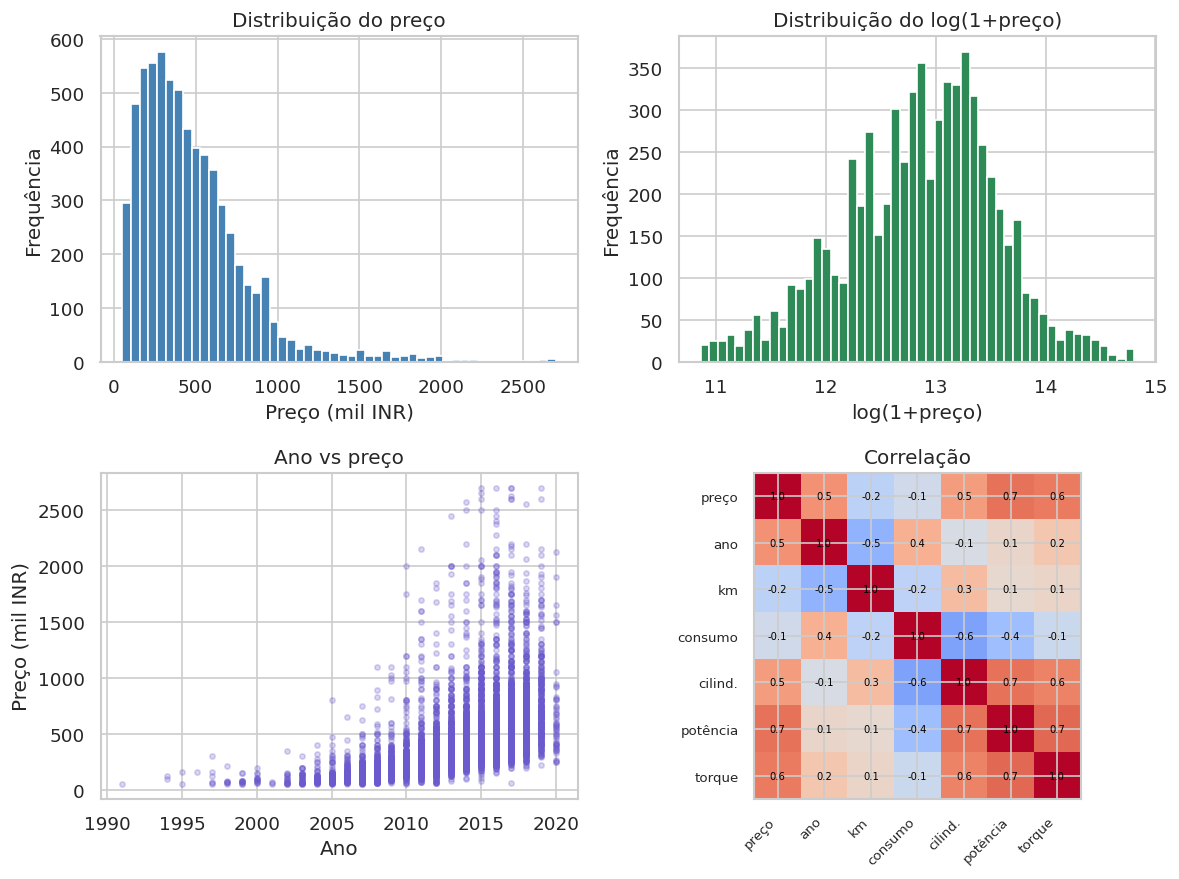
\includegraphics[width=\columnwidth]{Figures/eda_overview.png}}
\caption{Análise exploratória: distribuição do preço e do seu logaritmo, relação entre ano e preço, e matriz de correlação entre atributos numéricos.}
\label{fig:eda}
\end{figure}

A redundância entre atributos foi confirmada por Análise de Componentes Principais sobre as variáveis numéricas padronizadas, excluindo o preço. Conforme o gráfico de variância da Fig.~\ref{fig:scree}, três componentes concentram cerca de 80\% da variância total; a primeira componente é dominada pelos atributos de motor, enquanto a quilometragem e o consumo ganham peso na segunda.

\begin{figure}[t]
\centerline{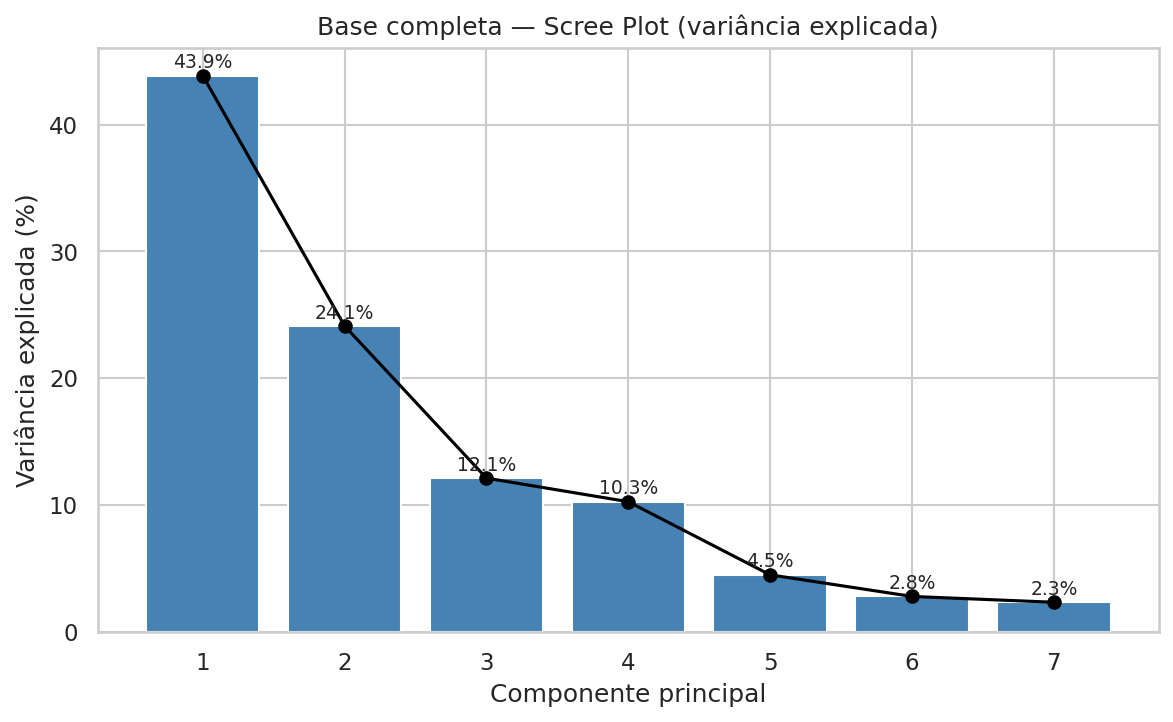
\includegraphics[width=0.9\columnwidth]{Figures/pca_scree.png}}
\caption{Variância explicada por componente principal e curva acumulada (\textit{scree plot}).}
\label{fig:scree}
\end{figure}

\subsection{Modelos}
Dada a forte assimetria à direita observada na distribuição do preço, optou-se por modelar a variável-alvo em escala logarítmica. Em vez de aprender o preço $y$ diretamente, cada modelo aprende uma função $g(\mathbf{x})$ sobre $z = \log(1 + y)$, com predição final obtida pela transformação inversa
\begin{equation}
\hat{y} = \exp\!\big(g(\mathbf{x})\big) - 1. \label{eq:logtarget}
\end{equation}
Como o preço é estritamente positivo e assimétrico, a transformação \eqref{eq:logtarget} aproxima a distribuição do alvo de uma normal, estabiliza a variância e converte relações multiplicativas em aditivas.

Para impedir o vazamento de informação, a partição treino--teste e a validação cruzada foram \textbf{agrupadas pelo nome do veículo}: amostras de um mesmo modelo, com especificações idênticas, jamais figuram simultaneamente em treino e teste. Resultaram 5.183 amostras de treino e 1.480 de teste, sem nenhuma sobreposição de grupos. Foram avaliados seis algoritmos, cujas configurações principais constam da Tabela~\ref{tab:config}: regressão linear, árvore de decisão, $k$-vizinhos mais próximos, gradient boosting, floresta aleatória --- com hiperparâmetros ajustados por busca em grade com validação cruzada agrupada --- e XGBoost. O procedimento de treino e avaliação é descrito no Algoritmo~\ref{alg:proc}.

\begin{table}[t]
\caption{Configuração Principal dos Modelos}
\begin{center}
\footnotesize
\begin{tabular}{ll}
\toprule
\textbf{Modelo} & \textbf{Configuração} \\
\midrule
Regressão linear & sem hiperparâmetros \\
Árvore de decisão & profundidade 12; mín. 5 amostras/folha \\
$k$-vizinhos & $k=7$; ponderação por distância \\
Gradient boosting & 150 árvores; prof. 3; taxa 0,08 \\
Floresta aleatória & 120 árvores; prof. 16; mín. 2/folha (busca em grade) \\
XGBoost & 300 árvores; prof. 4; taxa 0,08; subamostragem 0,9 \\
\bottomrule
\end{tabular}
\label{tab:config}
\end{center}
\end{table}

\begin{figure}[t]
\centering
\fbox{\begin{minipage}{0.92\columnwidth}
\footnotesize
\textbf{Algoritmo 1.} Treino e avaliação comparativa \label{alg:proc}
\begin{enumerate}\setlength{\itemsep}{1pt}
\item Particionar os dados em treino (80\%) e teste (20\%), agrupando pelo veículo.
\item Para cada modelo do conjunto de candidatos:
\begin{enumerate}\setlength{\itemsep}{1pt}
\item Encadear pré-processamento e modelo com alvo em escala log, Eq.~\eqref{eq:logtarget}.
\item Estimar o desempenho por validação cruzada agrupada de cinco dobras.
\item Registrar média e desvio-padrão das métricas entre as dobras.
\item Reajustar no treino completo e avaliar no conjunto de teste.
\end{enumerate}
\item Selecionar o melhor modelo pela menor raiz do erro quadrático médio em validação cruzada.
\item Comparar os dois melhores por teste estatístico, interpretar e analisar resíduos.
\end{enumerate}
\end{minipage}}
\end{figure}

\subsection{Avaliação}
A avaliação empregou validação cruzada de cinco dobras sobre o conjunto de treino. Sejam $y_i$ o preço real, $\hat{y}_i$ o preço previsto, $\bar{y}$ a média dos preços e $n$ o número de amostras. Foram adotadas quatro métricas complementares:
\begin{align}
\text{MAE} &= \frac{1}{n}\sum_{i=1}^{n} |y_i - \hat{y}_i|, \label{eq:mae}\\
\text{RMSE} &= \sqrt{\frac{1}{n}\sum_{i=1}^{n} (y_i - \hat{y}_i)^2}, \label{eq:rmse}\\
\text{MAPE} &= \frac{1}{n}\sum_{i=1}^{n} \frac{|y_i - \hat{y}_i|}{|y_i|}, \label{eq:mape}\\
R^{2} &= 1 - \frac{\sum_{i=1}^{n}(y_i - \hat{y}_i)^2}{\sum_{i=1}^{n}(y_i - \bar{y})^2}. \label{eq:r2}
\end{align}
A significância da diferença entre os dois melhores modelos foi avaliada por um teste $t$ pareado sobre o $R^{2}$ das cinco dobras. Métricas de classificação, como acurácia e curva ROC, não se aplicam, por se tratar de um problema de regressão.

\section{Experimentos e Resultados}

A Tabela~\ref{tab:resultados} apresenta o desempenho dos seis modelos, conforme o fluxo da Fig.~\ref{fig:pipeline}. Os métodos de comitê apresentaram os menores erros. O \textbf{XGBoost} foi o mais acurado em todas as métricas, com $R^{2}=0{,}916$ no conjunto de teste, erro absoluto médio de INR\,65,0 mil e erro percentual de 16,2\%, seguido pelo gradient boosting ($R^{2}=0{,}896$). A Fig.~\ref{fig:comp} sintetiza visualmente esse ordenamento.

\begin{table*}[t]
\caption{Desempenho dos Modelos na Validação Cruzada Agrupada (CV, 5 Dobras) e no Conjunto de Teste}
\begin{center}
\begin{tabular}{lrrrrrrr}
\toprule
\textbf{Modelo} & \textbf{CV MAE} & \textbf{CV RMSE} & \textbf{CV R\textsuperscript{2}} & \textbf{CV MAPE} & \textbf{Teste RMSE} & \textbf{Teste MAPE} & \textbf{Teste R\textsuperscript{2}} \\
\midrule
Regressão linear      & 79.079 & 133.910 & 0,847 & 17,6\% & 125.663 & 17,5\% & 0,877 \\
Árvore de decisão     & 91.814 & 155.336 & 0,795 & 21,3\% & 160.497 & 21,4\% & 0,799 \\
$k$-vizinhos mais próximos & 86.136 & 145.094 & 0,818 & 19,7\% & 138.288 & 19,8\% & 0,851 \\
Gradient boosting     & 75.698 & 123.926 & 0,869 & 17,2\% & 115.459 & 17,0\% & 0,896 \\
Floresta aleatória (ajustada) & 78.360 & 132.325 & 0,850 & 18,0\% & 122.037 & 17,8\% & 0,884 \\
XGBoost               & \textbf{71.839} & \textbf{117.532} & \textbf{0,881} & \textbf{16,5\%} & \textbf{103.740} & \textbf{16,2\%} & \textbf{0,916} \\
\bottomrule
\multicolumn{8}{l}{\footnotesize MAE e RMSE em rúpias indianas (INR). Em negrito, o melhor valor de cada métrica.}
\end{tabular}
\label{tab:resultados}
\end{center}
\end{table*}

A regressão linear, mesmo após a transformação logarítmica, e a árvore de decisão isolada figuraram entre os modelos mais limitados; esta última foi a mais sensível à partição agrupada ($R^{2}=0{,}799$), coerente com sua natureza de alta variância. Esse ordenamento responde à \textbf{PP2}: os comitês superam o \textit{baseline} linear em cerca de quatro pontos percentuais de $R^{2}$ e reduzem o erro percentual de 17,5\% para 16,2\%.

\begin{figure}[t]
\centerline{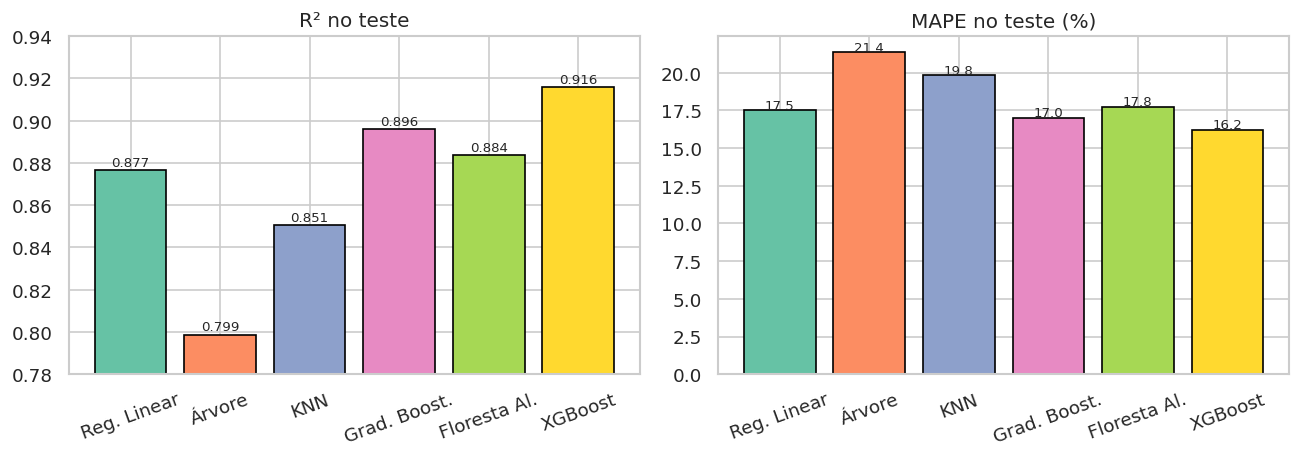
\includegraphics[width=\columnwidth]{Figures/model_comparison.png}}
\caption{Comparação do coeficiente de determinação e do erro percentual absoluto médio dos seis modelos no conjunto de teste.}
\label{fig:comp}
\end{figure}

\subsection{Significância Estatística}
Para verificar se a vantagem do XGBoost sobre o gradient boosting é consistente, aplicou-se um teste $t$ pareado sobre o $R^{2}$ das cinco dobras da validação cruzada. Obteve-se $t = 2{,}90$ e $p = 0{,}044$, valor inferior a 0,05; conclui-se que a superioridade do XGBoost é \textbf{estatisticamente significativa}. Esse resultado endereça a \textbf{PP3}: o ganho de acurácia do XGBoost não é fruto do acaso amostral. Ressalta-se ainda que os comitês apresentaram os menores desvios-padrão de $R^{2}$ entre as dobras (XGBoost $0{,}881 \pm 0{,}029$; gradient boosting $0{,}869 \pm 0{,}025$), contra $0{,}795 \pm 0{,}033$ da árvore isolada, evidenciando predições mais consistentes.

\subsection{Benchmarking com a Literatura}
A Tabela~\ref{tab:bench} posiciona os resultados obtidos frente a estudos correlatos. Como os conjuntos de dados diferem, a comparação é qualitativa; ainda assim, o $R^{2}$ de 0,916 alcançado situa-se acima da faixa tipicamente reportada (0,77 a 0,93), o que sugere boa competitividade da abordagem, sobretudo por adotar partição agrupada, condição mais rigorosa e menos frequente na literatura.

\begin{table}[t]
\caption{Comparação com Trabalhos Relacionados (R\textsuperscript{2} no Teste)}
\begin{center}
\footnotesize
\begin{tabular}{lll}
\toprule
\textbf{Trabalho} & \textbf{Melhor modelo} & \textbf{R\textsuperscript{2}} \\
\midrule
Itm \textit{et al.} \cite{itm2025} & XGBoost & $\approx$ 0,87 \\
Revolutionizing \cite{revolution} & XGBoost & $\approx$ 0,87--0,93 \\
How much \cite{howmuch} & Floresta aleatória & $\approx$ 0,83 \\
Este trabalho & XGBoost & \textbf{0,916} \\
\bottomrule
\multicolumn{3}{l}{\footnotesize Conjuntos de dados distintos; comparação qualitativa.}
\end{tabular}
\label{tab:bench}
\end{center}
\end{table}

\subsection{Interpretação por Permutação}
A importância das variáveis foi avaliada por permutação --- que mede a queda de $R^{2}$ ao embaralhar cada atributo no conjunto de teste --- método mais robusto que a importância por impureza. Conforme a Fig.~\ref{fig:importance}, respondendo à \textbf{PP1}, o ano do veículo é o preditor dominante (queda de 0,49 no $R^{2}$), seguido da potência (0,29), do torque (0,09) e, notavelmente, da marca (0,07), cuja relevância é maior do que a sugerida pela importância por impureza. A cilindrada, a quilometragem e a transmissão completam o conjunto de atributos influentes. Esse resultado é coerente com a Análise de Componentes Principais, na qual os atributos de motor dominam a primeira componente.

\begin{figure}[t]
\centerline{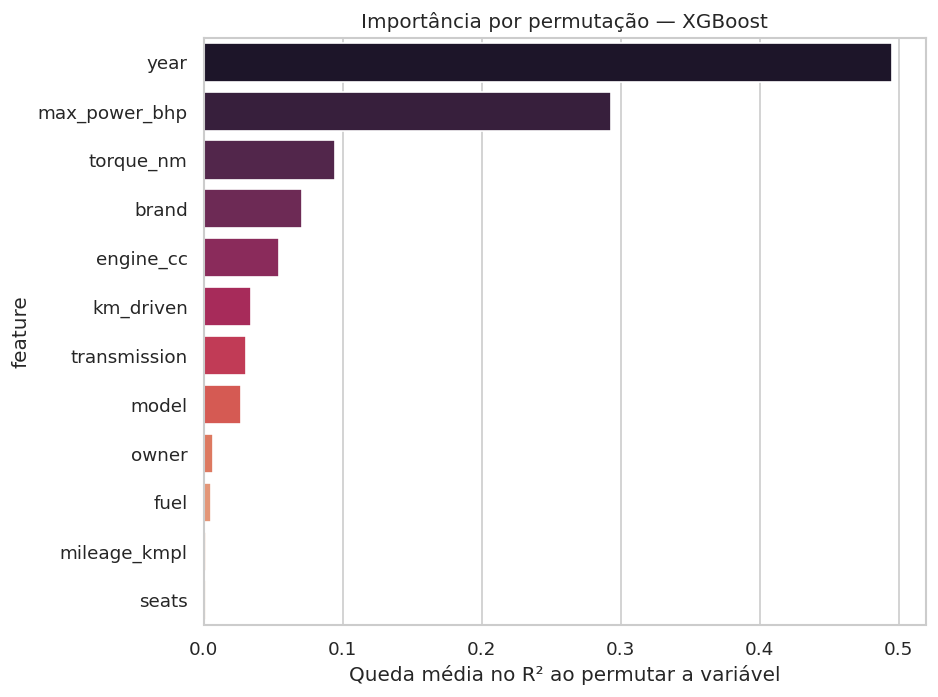
\includegraphics[width=0.95\columnwidth]{Figures/permutation_importance.png}}
\caption{Importância por permutação das variáveis segundo o melhor modelo (XGBoost): queda média no $R^{2}$ ao permutar cada atributo.}
\label{fig:importance}
\end{figure}

A análise de resíduos do melhor modelo é apresentada na Fig.~\ref{fig:residuos}. A nuvem de resíduos está aproximadamente centrada em zero e sua distribuição é simétrica, o que indica ausência de viés sistemático relevante; o treino em escala logarítmica mitigou boa parte da heterocedasticidade típica de variáveis de preço.

\begin{figure}[t]
\centerline{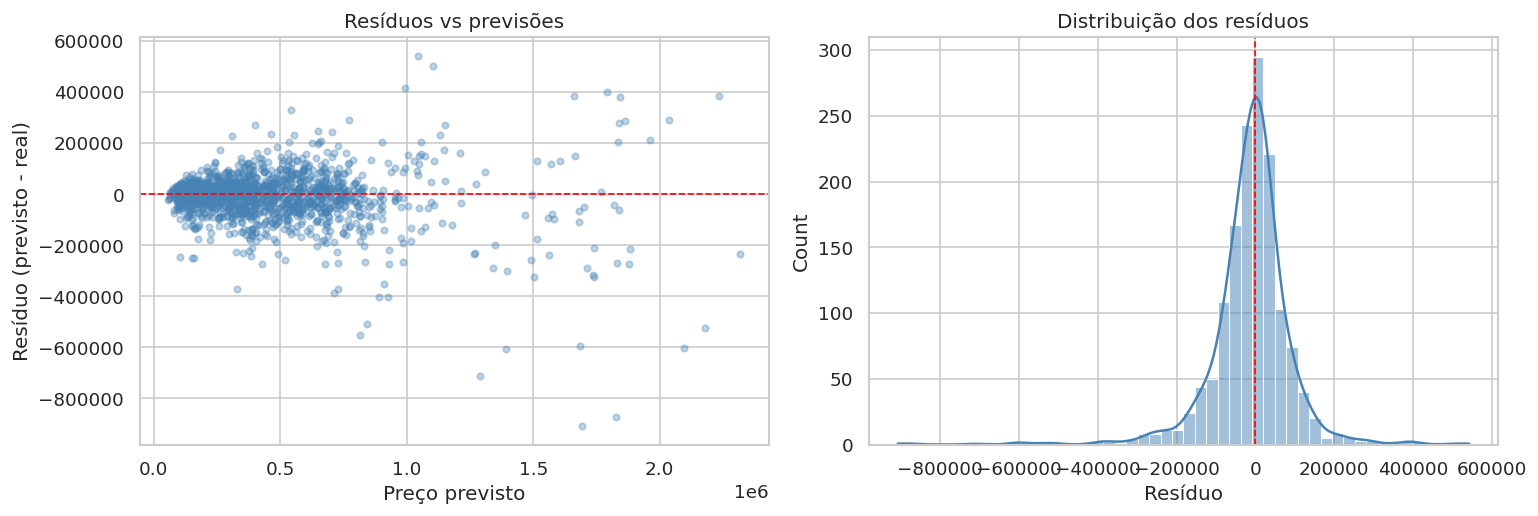
\includegraphics[width=\columnwidth]{Figures/residuals.png}}
\caption{Análise de resíduos do melhor modelo: dispersão dos resíduos em função das predições (esquerda) e distribuição dos resíduos (direita).}
\label{fig:residuos}
\end{figure}

\section{Discussão}

A comparação entre as famílias de modelos ilustra didaticamente o dilema viés--variância. A regressão linear exibe alto viés (subajuste): é estável, porém limitada, pois o efeito da potência sobre o preço varia conforme a marca e a categoria do veículo --- interação que um modelo aditivo não representa. O método de vizinhança sofre com a maldição da dimensionalidade, agravada pela codificação \textit{One-Hot}. A árvore de decisão isolada, de alta variância, foi a mais penalizada pela partição agrupada. Os comitês corrigem essa fragilidade: a floresta aleatória reduz a variância pela média de árvores descorrelacionadas, enquanto o gradient boosting e o XGBoost reduzem o viés de forma sequencial; o XGBoost beneficia-se ainda de regularização explícita, o que explica seu desempenho superior e estatisticamente significativo.

A interpretação por permutação corrige uma limitação importante da importância por impureza, que tende a superestimar variáveis contínuas e de alta cardinalidade e a subdimensionar variáveis categóricas fragmentadas pela codificação \textit{One-Hot}. Ao permutar atributos no conjunto de teste, obteve-se uma estimativa mais fiel, na qual a marca emergiu como fator relevante. Ainda assim, atributos de motor fortemente correlacionados podem repartir a importância entre si, de modo que os valores devem ser lidos como tendências.

\subsection{Limitações}
Destacam-se quatro limitações: (i) os dados restringem-se a um único mercado, o que limita a generalização externa; (ii) o nome do veículo foi reduzido à marca e ao modelo, descartando informação de versão; (iii) o conjunto apresenta desbalanceamento entre marcas; e (iv) não foi realizada validação temporal, embora preços variem ao longo do tempo.

\subsection{Contribuições}
Do ponto de vista acadêmico, a contribuição reside na integração, em um fluxo reprodutível, da partição agrupada contra vazamento, do ajuste de hiperparâmetros, da comparação por validação cruzada com teste estatístico e da interpretação por permutação. Do ponto de vista prático, o erro percentual médio de 16,2\%, no contexto de preços médios superiores a INR\,480 mil, e o baixo custo de inferência do XGBoost viabilizam a aplicação do modelo em cenários de precificação assistida.

\section{Conclusão e Trabalhos Futuros}
Foi desenvolvido um fluxo completo e robusto de previsão de preços de carros usados, da limpeza de 8.128 registros à comparação de seis algoritmos por validação cruzada agrupada. O XGBoost obteve o melhor desempenho, com coeficiente de determinação de 0,916 no conjunto de teste, superando de forma estatisticamente significativa o gradient boosting, e tendo o ano, a potência e o torque como preditores dominantes. Em resposta às perguntas de pesquisa, confirmou-se a relevância dos atributos de idade e mecânica (PP1), a superioridade dos comitês sobre o \textit{baseline} (PP2) e a vantagem do XGBoost em acurácia e estabilidade (PP3).

Como trabalhos futuros, propõem-se: a adoção de valores SHAP \cite{shap} para interpretação local; a inclusão de algoritmos adicionais, como \textit{LightGBM} e redes neurais tabulares; o emprego de validação temporal; e a quantificação da incerteza das predições por meio de intervalos de confiança.

\begin{thebibliography}{00}
\bibitem{cardekho} CarDekho/Kaggle, ``Vehicle dataset --- Car details v3,'' conjunto de dados público de anúncios de carros usados, 2020. [Online].
\bibitem{hastie} T. Hastie, R. Tibshirani, and J. Friedman, \textit{The Elements of Statistical Learning}, 2nd ed. New York: Springer, 2009.
\bibitem{breiman} L. Breiman, ``Random forests,'' \textit{Machine Learning}, vol. 45, no. 1, pp. 5--32, 2001.
\bibitem{friedman} J. H. Friedman, ``Greedy function approximation: A gradient boosting machine,'' \textit{Annals of Statistics}, vol. 29, no. 5, pp. 1189--1232, 2001.
\bibitem{chen2016} T. Chen and C. Guestrin, ``XGBoost: A scalable tree boosting system,'' in \textit{Proc. 22nd ACM SIGKDD}, 2016, pp. 785--794.
\bibitem{itm2025} ``Machine learning optimization and challenges in used car price prediction,'' \textit{ITM Web of Conferences}, 2025.
\bibitem{preowned2023} ``Pre-owned car price prediction by employing machine learning techniques,'' 2023.
\bibitem{revolution} ``Revolutionizing the used car market: Predicting prices with XGBoost,'' 2024.
\bibitem{howmuch} N. Pal \textit{et al.}, ``How much is my car worth? A methodology for predicting used cars' prices using random forest,'' in \textit{Proc. Future of Information and Communication Conf.}, 2018.
\bibitem{mobileapp2022} ``Machine learning-powered mobile app for predicting used car prices,'' in \textit{Proc. ACM Conf.}, 2022.
\bibitem{ritthesis} ``Used cars price prediction and valuation using data mining techniques,'' M.S. thesis, Rochester Institute of Technology, 2022.
\bibitem{shap} S. M. Lundberg and S.-I. Lee, ``A unified approach to interpreting model predictions,'' in \textit{Adv. Neural Inf. Process. Syst. (NeurIPS)}, 2017.
\bibitem{pco213} G. Bernardes Vitor, ``PCO213 --- Aprendizado de Máquina e Mineração de Dados,'' Universidade Federal de Itajubá, 2026.
\end{thebibliography}

\end{document}
